~\chapter{~\emph{ARHydra}}
\label{cap:arhydra}
	%\epigraph{`` The most profound technologies are those that disappear.''}{Mark Weiser}
	
		
	O \textit{smart space} pode ser composto por uma grande variedade de dispositivos, os quais
	disponibilizam recursos ao ambiente. Por sua vez, esses recursos devem ser utilizados para suprir
	as necessidades do usuário e auxiliar na execução de suas tarefas da melhor forma possível.
	Adicionalmente, o ambiente poderá oferecer ao usuário a possibilidade de seleção do recurso a ser
	utilizado na execução de uma tarefa. Dentro desse contexto, a aplicação Hydra (apresentado na
	seção \ref{sec:hydra}), utilizando o \textit{middleware uOS} (seção \ref{sec:uos}), possibilita ao
	usuário escolher e utilizar um determinado recurso disponível no ambiente.
	
	Devido a grande volatilidade e a quantidade de dispositivos dentro do ambiente inteligente, a
	aplicação ARHydra (apresentada na seção \ref{sec:arHydra}) utiliza os recursos providos pela
	Realidade Aumentada e os objetivos do \textit{uOS} auxiliando o usuário na visualização e seleção
	dos recursos presentes no ambiente inteligente.
	
	\section{O \textit{middleware} uOS}
\label{sec:uos}
	 
	O \textit{middleware uOS}, projeto do grupo de pesquisa \textit{UnBiquitous} da Universidade de
	Brasília, tem como objetivo a integração das aplicações no ambiente inteligente e foca na
	adaptabilidade dos serviços presentes nos mais diversos dispositivos. Desta forma, os serviços
	passam a ser compartilhados de uma forma menos intrusiva \cite{buzeto}. Conforme apresentado na
	figura~\ref{fig:dsoa}, o \textit{middleware uOS} atua como uma camada entre as aplicações
	e~\textit{drivers}.
	
	\begin{figure}[htb]
		\centering 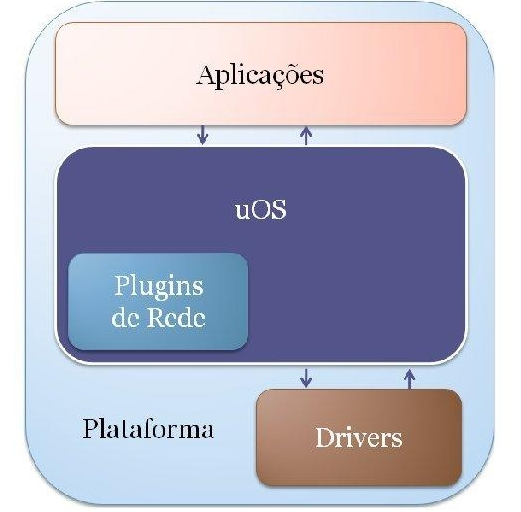
\includegraphics[scale=.35]{figuras/cap2/dsoa.jpg}
		\caption{\textit{Middleware uOS~\cite{buzeto}.}}
		\label{fig:dsoa} 
	\end{figure}
	 
	O \textit{uOS} segue os conceitos propostos pela ~\textit{DSOA} (\textit{Device Service Oriented
	Architecture}) para modelagem do ambiente inteligente. Nessa arquitetura são definidos o modelo
	de comunicação a ser utilizado, implementando algumas características definidas pelo
	~\textit{SOA (Service Oriented Architecture)}~\cite{buzeto_11}. Por causa da diversidade e capacidade de
	processamento dos diversos dispositivos presentes no \textit{smart space}, foi criado um conjunto
	de protocolos para a computação ubíqua, implementada sobre o ~\textit{middleware uOS}, denominada de ~\textit{uP
 	(Ubiquitous Protocols)}, viabilizando uma maneira simplificada e padronizada para a troca de
 	informações entre esses dispositivos. O \textit{uP} permite uma interação entre os dispositivos,
 	levando-se em consideração a heterogeneidade das plataformas, os diferentes modelos de comunicação
 	e interação com o ambiente. Desta forma, o \textit{uP} possibilita a descoberta de novos
 	dispositivos no ambiente e a representação dos recursos através de \textit{drivers}.
	
	O \textit{uOS} foi desenvolvido na linguagem JAVA, possibilitando a utilização do mesmo nos mais
	diversos dispositivos que a ofereçam suporte. Ele se encontra disponível em duas versões: uma
	\textit{mobile}, sob a plataforma JME (\textit{Java Micro Edition}), e uma seguindo a plataforma
	JSE (\textit{Java Standart Edition}). Esta última foi também portada para a utilização em
	dispositivos Android. Viabilizando sua utilização tanto em dispositivos limitados (usando a
	plataforma \textit{mobile} ou Android) à outros mais capazes.
	

	\section{A aplicação Hydra}
\label{sec:hydra}
	
	
	Na visão da \textit{ubicomp}, o \textit{smart space} é composto por diversos dispositivos que
	fornecem uma gama de recursos e funcionalidades. É plausível de se esperar que muitos destes
	recursos sejam equivalentes entre si, como a existência de várias telas a disposição. Com tantas
	opções espera-se que um ambiente inteligente possibilite ao usuário escolher aquela que melhor lhe
	atende na tarefa sendo realizada. É neste cenário que a aplicação Hydra entra em cena. Fazendo uso
	da plataforma provida pelo \textit{middleware uOS}, esta aplicação permite que o usuário
	redirecionar os recursos de sua máquina para outros mais adequados no ambiente \cite{almeida}.

    Para melhor entender a atuação da Hydra no ambiente considere o seguinte exemplo de uso:
	 
	O ambiente é dotado dos seguintes dispositivos:
	 
	
	\begin{enumerate}
		\item Macbook e o \textit{notebook} HP disponibilizam os recursos de \textit{webcam}, saída de
		vídeo, mouse e teclado;
		\item \textit{Laptop} Dell disponibiliza somente os recursos de saída de vídeo, mouse e teclado;
		\item \textit{Smartphone} Galaxy SII disponibiliza os recursos de câmera, mouse e teclado;
		\item \textit{SmartTV} disponibiliza os recursos de saída de vídeo. 
	\end{enumerate}
	
	A seguir temos um exemplo de interação neste ambiente utilizando a Hydra:

	\begin{quote}
	
		\it 	
		Inicia-se uma reunião cujo propósito é alinhar os conhecimentos a respeito dos projetos do grupo 
		UnBiquitous, discutir as soluções propostas e apresentar os artigos base para os projetos. Os
		participantes da reunião são Marcelo (dono do notebook HP), Bruno (dono do smartphone Galaxy SII), Ricardo (dono do
		Macbook) e Fabrício (dono laptop Dell).
		
		Para facilitar a visualização dos tópicos a serem discutidos, Fabrício como líder do projeto,
		instalou a aplicação Hydra em seu laptop e redirecionou a tela do laptop para a SmartTV. Os
		demais dispositivos estão utilizando uma instância do middleware uOS, disponibilizando seus
		recursos ao ambiente.

		Fabrício mostra a pauta da reunião. Após a discussão dos primeiros tópicos, Ricardo sente a
		necessidade de complementar alguns tópicos apresentados. Ricardo então pede ao Fabrício que
		redirecione o recurso de teclado do laptop Dell para seu Macbook. Após acrescentar os novos
		tópicos, Ricardo pede ao Fabrício que libere o recurso do teclado, para que seja utilizado o
		teclado do laptop do Fabríco novamente. Bruno percebe a necessidade de apontar algumas questões
		nos novos tópicos criados pelo Ricardo e solicita ao Fabrício que o recurso de mouse seja
		utilizado em seu celular. Com os avanços dos apontamentos feitos pelo Bruno, Marcelo
		decide mostrar um vídeo que lhe chamou a atenção. Solicita então o uso do recurso de saída de vídeo para
		que possa exibi-lo na SmartTV. Após o término da exibição do vídeo o grupo encerra as discussões
		e finaliza a reunião.

	\end{quote}
		
	Ao final da reunião, a aplicação Hydra proporcionou uma visão diferente no ~\textit{laptop} Dell
	pertencente ao Fabrício devido ao redirecionamento dos recursos. Neste, os recursos de saída de
	vídeo e \textit{mouse} estão direcionados para outros dispositivos no ambiente. Desta forma o
	~\textit{laptop} do Fabrício pode ser visto como uma composição dos recursos que estão distribuídos
	no ambiente. 
	
	Através desse exemplo foi possível observar que os dispositivos foram redirecionados de uma
	forma manual, partindo de uma necessidade específica. No entanto, a Hydra pode implementar
	inteligências que simplifiquem essa seleção e o redirecionamento dos recursos.
	
~\subsection{Recursos}

	Com o propósito de preservar a invisibilidade do sistema, a interação do usuário com os recursos
	pode acontecer de três formas distintas:
	
	\begin{itemize}
	  \item Interação direta
	  
	  		Esta interação possibilita ao usuário escolher qual dispositivo será utilizado, levando
	  		em consideração as vantagens e desvantagens de cada recurso.
	  
	  \item Interação sugerida
	  
	  		O sistema apresenta, de forma organizada, as possibilidades disponíveis compatíveis com a
	  		necessidade do usuário em um determinado momento, sendo esta implementada através de um
	  		mecanismo de inteligência.
	  		
	  \item Interação automática
	  
	  		Nesta interação, o sistema leva em consideração a sensibilidade do contexto para selecionar,
	  		automaticamente, o dispositivo que mais adeque ao propósito de resolução da tarefa intencionada.
	  		
	\end{itemize}
	
	
	A Hydra implementa a Interação Sugerida seguindo os conceitos apresentados pela \textit{DSOA}.
	Ela oferece suporte para quatro tipos de recursos, sendo estes definidos no ambiente através de
	\textit{UpDriver's}:
	
	\begin{enumerate}
	  \item \textit{Mouse}
		
			Este \textit{driver} provê uma abstração para comandos enviados por um apontador. Os eventos
			gerados por esse \textit{driver}, como por exemplo um clique duplo, são enviados ao destinatário
			através de eventos compostos por mensagens. Estes eventos são reconhecidas na Hydra e a
			movimentação do ponteiro na Hydra é feita com o uso da classe \textit{Robot}.
			
			São exemplos de serviços disponibilizados por esse recurso: 
			\begin{itemize}
			  \item posicionamento do ponteiro;
			  \item clique simples;
			  \item duplo clique;
			  \item clique com o botão direito;
			  \item	\textit{scroll}. 
			\end{itemize}
		
	  		A implementação desse recurso está disponível para as versões JSE (\textit{Java Standard Edition)} 
	  		e JME (\textit{Java Micro Edition}).

	  \item Teclado
	  		
	  		Esse recurso possui um comportamento similar ao \textit{mouse}, no que diz respeito
	  		envio dos eventos capturados. Este por sua vez, implementa o reconhecimento de
	  		eventos para pressionamentos, simples e simultâneo, e liberação de teclas, realizando
	  		capturas para:
	  		
	  		\begin{itemize}
	  		  \item Caracteres, maiúsculos ou minúsculos;
	  		  \item Números, de 0 a 9;
	  		  \item Comandos de teclado (\textit{shift}, \textit{control} e \textit{alt});
	  		  \item Teclas de funções  (F1 a F12);
	  		  \item Botões do teclado numérico.
	  		\end{itemize}
	
	  		Devido a diversidade de leiautes  configuráveis pelo teclado, os eventos capturados podem ser
	  		interpretados pela Hydra de uma forma diferente. Um exemplo desse comportamento pode ser
	  		observado no evento de captura da tecla ``ç'', para o leiaute do teclado no padrão ABNT2.
	  		Neste caso, para o padrão ABNT, o evento que apresenta a tecla ``ç'' é configurado como uma
	  		combinação de eventos de outras teclas. Essas diferenças são esperadas e podem serem corrigidas
	  		através da configuração do novo leiaute.
	  		
	  		As mensagens recebidas pela Hydra são traduzidos em comandos, que por sua vez são emulados
	  		utilizando a classe \textit{Robot}.
	  		
	  \item Tela
	  	
	  		Esse recurso utiliza a classe \textit{Robot} para capturar as imagens da tela, ao qual
	  		posteriormente será sequencia e transformada em um formato de vídeo adequado para transmissão.
	  		A transmissão do ~\textit{streaming} de dados é feita através do protocolo RTP (\textit{Real
	  		Time Protocol}) utilizando o JMF (\textit{Java Media Framework}).

	  		Após o recebimento do conteúdo na Hydra, o \textit{streaming} de dados é interpretado, 
	  		reconstruído e posteriormente exibido na tela utilizada pela aplicação Hydra.
	  	
	  \item Câmera
	  
			De modo análogo a funcionalidade de tela, este \textit{driver} utiliza o protocolo RTP para
			realizar a transmissão do \textit{streaming} de dados. Adicionalmente, este \textit{driver}
			disponibiliza os serviços de seleção e ativação de câmeras presentes no dispositivo. Após a
			detecção das câmeras e da seleção de qual câmera utilizar, a aplicação Hydra receberá o
			\textit{streaming} de dados enviados pela câmera escolhida e exibirá o conteúdo recebido em uma
			nova janela na tela utilizada pela Hydra.
		
	\end{enumerate}
	
	Com o suporte para esses conjunto de recursos, a Hydra consegue abranger uma boa gama de
	cenários de uso. A maioria dos recursos estão classificados em um dos tipos de recursos
	suportados pela Hydra, possibilitando assim o redirecionamento de diversos recursos presentes no
	ambiente inteligente.
	

	\section{Incrementando a Hydra com a Realidade Aumentada}
\label{sec:arHydra}

	Conforme visto, a Hydra auxilia no redirecionamento de recursos de um dispositivo para outros mais
	adequados no ambiente. Sua interação é feita de maneira sugerida, de forma que são exibidos para a
	seleção do usuário apenas aqueles que lhe são compatíveis. Nesta abordagem, cabe ao usuário
	realizar a ligação entre o nome do dispositivo exibido nas opções e o recurso que deseja utilizar.	
	No entanto, o usuário pode ter dificuldades de associar o nome exibido e ao dispositivo contendo o
	recurso desejado.
	
	A figura \ref{fig:sala_computadores} mostra uma sala com computadores com características físicas
	semelhantes, numerados de 1 à 12. Considere que um usuário esteja utilizando o computador de
	número 4 e deseje utilizar um recurso específico de um outro computador (assuma que todos os
	computadores estejam disponibilizando seus recursos no ambiente). A Hydra mostrará uma lista de
	recursos passíveis de redirecionamento e ficará aguardando a seleção de um dispositivo. Suponha que o
	recurso desejado esteja disponível no computador de número 10 e o usuário o selecione. Nesse
	momento, o usuário terá que identificar qual computador foi selecionado na lista fornecida pela
	Hydra. No entanto, como há uma grande similaridade nas características físicas, o usuário terá
	dificuldades de associar o nome exibido, pela lista da Hydra, ao equipamento selecionado.
	
	\begin{figure}[htb]
		\centering 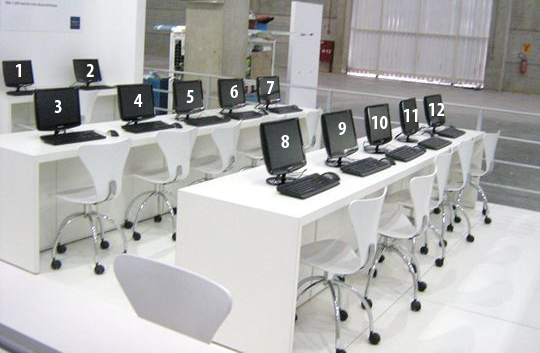
\includegraphics[scale=0.65]{figuras/cap3/sala_computadores.png}
		\caption{\textit{Sala com computadores.}}
		\label{fig:sala_computadores} 
	\end{figure}


    A ARHydra (\textit{Augmented Reality Hydra}) visa amenizar esta tarefa fazendo uso de técnicas de
    Realidade Aumentada. A inserção de informações através de objetos virtuais facilitará na
    identificação dos dispositivos no ambiente inteligente. Os dispositivos serão mapeados através de
    marcadores estrategicamente localizados no dispositivo. De modo que, novas informações a
    respeito dos recursos disponibilizados pelo dispositivo fossem apresentadas para o usuário no
    momento de sua localização.
    
    Esse novo meio de visualização dos recursos proverá uma nova forma de interação entre o
    usuário e o ambiente inteligente. Desta forma, a utilização das facilidades de redirecionamento
    de recursos provida pela Hydra pode ser incrementada com uma visualização, e localização,
    simplificada destes.
    
\subsection{Marcadores na ARHydra}

	Aplicações para a realidade aumentada utilizam marcadores com características próprias, como é
	o caso das aplicações ARToolkit e ARTag. A maior parte dos trabalhos que utilizam esses
	marcadores, associam o código de identificação extraído do marcador a um objeto virtual
	pré-definido. Essa relação causa uma dependência de um mapeamento prévio de todos os objetos 
	virtuais e seus respectivos códigos de identificação, proporcionando uma limitação na interatividade 
	entre novos marcadores.
	
	A ARHydra segue uma estratégia diferente. Utiliza características que favoreçam o reconhecimento e
	a extração de informações através de seus marcadores, sem a necessidade de uma tabela de
	mapeamento. Esse comportamento híbrido proporciona uma interatividade na identificação dos
	marcadores, uma vez que a disponibilidade dos recursos dependem dos dispositivos presentes no
	ambiente.
	 
	A escolha do código QRCode, para identificação dos marcadores, baseia-se na possibilidade de
	inserção de caracteres alfanuméricos, na rápida leitura e na tolerância a erros oferecidas por
	esse código bidimensional. Possibilitando assim, uma forma simplificada para a extração da
	identificação dos dispositivos no ambiente inteligente. 
	
	A figura \ref{fig:arhydra_marcador} exemplifica o marcador utilizado pela ARHydra. Na primeira
	parte da figura é apresentado um marcador utilizado pela aplicação ARToolkit. Em seguida, um
	código QRCode responsável por armazenar alguma informação relevante a respeito do dispositivo. A
	junção dos mesmos formará um marcador constituído de bordas pretas, aos quais delimitam o marcador
	e favorecem uma forma rápida de localização, e o QRCode no centro do marcador, responsável pela
	identificação do marcador.
	
	\begin{figure}[h]
		\centering \includegraphics[scale=0.5]{figuras/cap3/marcador_arHydra.png}
		\caption{\textit{Marcador utilizado na ARHydra.}}
		\label{fig:arhydra_marcador} 
	\end{figure}
	
\subsection{Interação no ambiente}

	Considere o seguinte exemplo de interação da ARHydra com o ambiente. Suponha um 
	\textit{smart space} composto por:
	
	\begin{enumerate}
	  \item Macbook: disponibiliza os recursos de \textit{webcam}, saída de vídeo, \textit{mouse} e
	  teclado;
	  \item \textit{Smartphone} Galaxy SII: disponibiliza os recursos de câmera, mouse e teclado;
	  \item iMac: disponibiliza os recursos de saída de vídeo, \textit{mouse} e teclado.
	\end{enumerate}
	
	No macbook terá uma aplicação utilizando o \textit{uOS} disponibilizando seus recursos através de
	\textit{UpDriver's}, sendo este dispositivo mapeado no ambiente através de um marcador reconhecido
	pela ARHydra. O \textit{smartphone} ficará responsável pela execução da aplicação ARHydra. Por
	fim, a aplicação Hydra será executada no iMac. 
	
	O uso dos marcadores, alinhado com a mobilidade com que o \textit{smartphone} pode interagir com o
	ambiente, faz com que a aplicação ARHydra seja utilizada no \textit{smartphone} do usuário. Essa
	interação possibilita ao usuário uma melhor forma de localização e seleção do recurso disponível.
	
	A figura \ref{fig:apresentacao_arhydra} exemplifica o uso de um marcador para identificar o dispositivo no
	ambiente. Como etapa inicial ilustrada através da figura \ref{fig:visualizacao_qrcode}, há uma
	busca por esse marcador inserido no ambiente, ao qual posteriormente será feito uma tentativa de
	reconhecimento para obtenção da informação contendo os recursos disponibilizados. Com a conclusão
	bem sucedida da etapa anterior, o os recursos serão apresentados ao usuário, conforme ilustrado na
	figura \ref{fig:visualizacao_obj}. Essa exibição é feita utilizando técnicas da realidade
	aumentada. Por fim, a aplicação ARHydra possibilita ao usuário escolher qual recurso deseja que
	seja redirecionado para a Hydra.
	
	\begin{figure}[htb]
		\centering
			\subfloat[Visualização do marcador]{
				\label{fig:visualizacao_qrcode}
				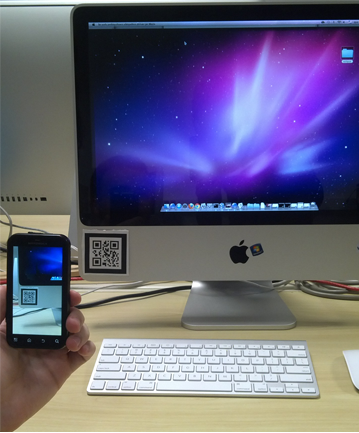
\includegraphics[width=0.45\textwidth]{figuras/cap3/visao_mac.png}
			}
			\subfloat[Visualização do objeto virtual]{
				\label{fig:visualizacao_obj}
				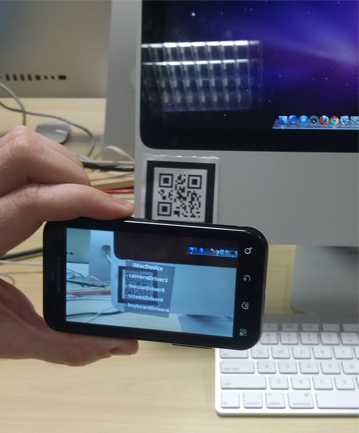
\includegraphics[width=0.45\textwidth]{figuras/cap3/visao_qrcode.png}
			}
		
		\caption{\textit{(a) Exemplo da visão do usuário para a busca do marcador do dispositivo. (b)
		Exemplo da visualização do objeto virtual apresentando os recursos disponíveis}}
		\label{fig:apresentacao_arhydra} 
	\end{figure}
	
	
	A interação da ARHydra no ambiente inteligente segue os passos observados na figura~\ref{fig:arhydra_interacao}:

	\begin{figure}[h] 
		\centering 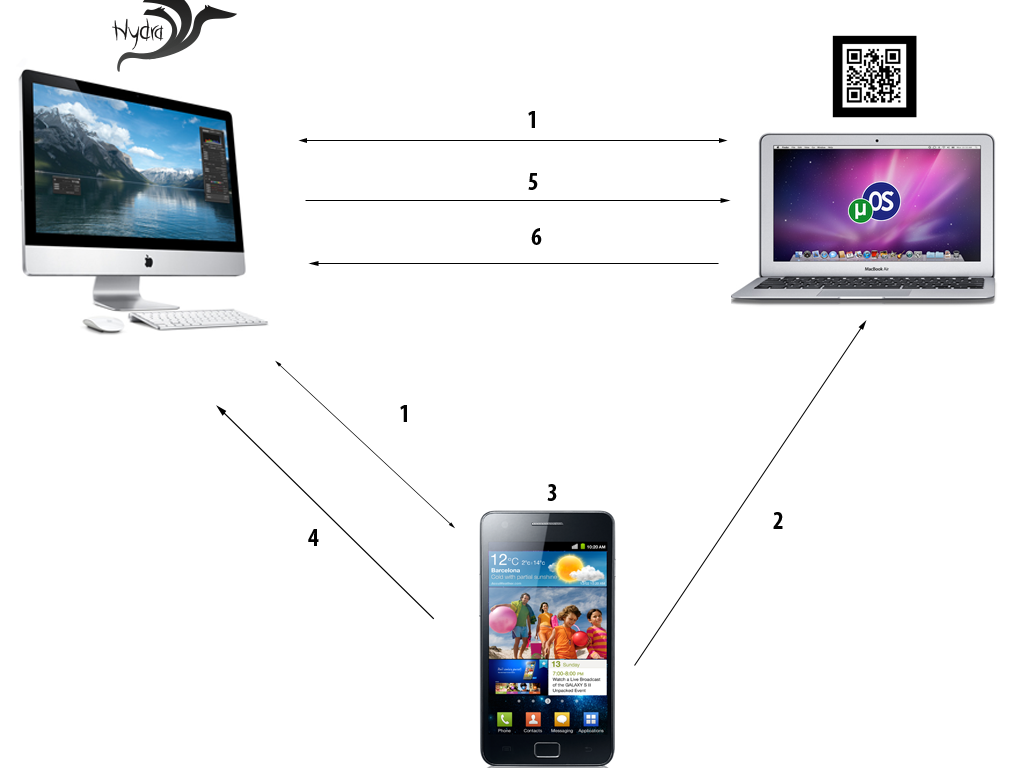
\includegraphics[scale=0.45]{figuras/cap3/integracao_arhydra.png}
		\caption{\textit{Integração Hydra com o ambiente.}}
		\label{fig:arhydra_interacao} 
	\end{figure}
	
	\begin{enumerate}
	  \item A Hydra implementa o mecanismo de descoberta de novos dispositivos e os registra os
	  dispositivos encontrados em sua base de dados;
	  
	  \item A ARHydra procura o marcador identificador do Macbook;
	  
	  \item Faz a reconhecimento e decodificação do marcador encontrado, busca os recursos disponíveis
	  do dispositivo e apresenta esses recursos na tela do \textit{smartphone} com os recursos
	  providos pela realidade aumentada, possibilitando ao usuário selecionar um recurso disponível.
	  
	  \item Caso o usuário selecione um recurso, a ARHydra faz uma requisição à Hydra para que
	  redirecione o recurso selecionado do Macbook para o uso na Hydra.
	  
	  \item A Hydra recebe a solicitação vinda do \textit{smartphone}, solicita o registro do
	  recurso selecionado para a aplicação do \textit{uOS} executada no Macbook.
	  
	  \item A partir desse momento, o recurso do Macbook selecionado pela ARHydra será redirecionado
	  para o iMac.
	\end{enumerate}

	Com isso, a aplicação ARHydra complementa a interação do usuário com a Hydra, auxiliando na
	identificação visual dos dispositivos e no redirecionamento dos recursos disponíveis. 
 	

	

